\subsection{Occlusion separates detection from staging}
\label{sec:occlusion-results}

All occlusion results in this subsection use the Laboro three-stage YOLO11n
detector of Table~\ref{tab:cross} on the 161 Laboro validation images, which
hold 1{,}996 annotated fruit. The ground-truth box is always the whole fruit,
so recall measures whether the model found the fruit. Stage accuracy is
computed only for the fruit that it found.

\begin{figure}[t]
  \centering
  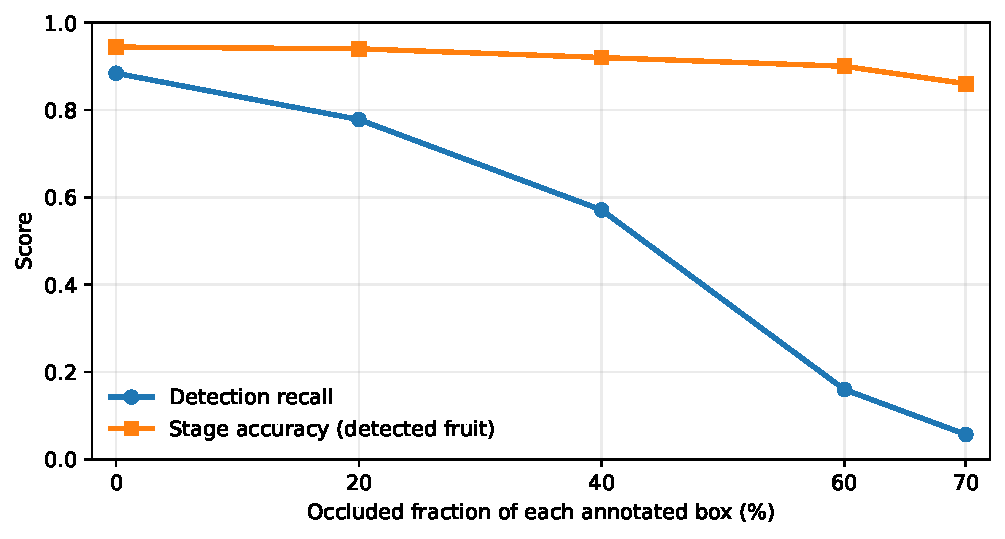
\includegraphics[width=\columnwidth]{occlusion_curve.pdf}
  \caption{Progressive synthetic occlusion. Detection recall collapses while
  maturity-stage accuracy among successfully detected fruit changes modestly.}
  \label{fig:occlusion-curve}
\end{figure}

Figure~\ref{fig:occlusion-curve} shows that occlusion affects detection more
than stage classification among detected fruit. Recall falls from 0.884 with
nothing hidden to 0.057 at 70\% hidden. Over the same range, stage accuracy for
the detected fruit falls from 0.944 to 0.860, while counting MAE rises from 1.25
to 2.99. The mean confidence of matched detections also falls from 0.840 to
0.506, bringing the remaining detections closer to the 0.25 threshold. At 40\%
hidden, recall is 0.52 for green, 0.63 for half-ripened, and 0.71 for fully
ripened fruit. Green fruit are the smallest fruit and are least distinct from
the surrounding leaves. The stage with the lowest unoccluded recall therefore
shows the largest loss.

\begin{table}[t]
\centering
\caption{Recall under synthetic occlusion for one detector, scored four ways.
Columns 2--3: same-image background strip, matched at IoU 0.5 and 0.3.
Column 4: flat black strip (IoU 0.5). Column 5: the mixed-data detector with
the background strip (IoU 0.5). The last two columns give counting MAE, which
does not depend on matching.}
\label{tab:occlusion-sweep}
\setlength{\tabcolsep}{4pt}
\begin{tabular}{rccccrr}
\toprule
& \multicolumn{4}{c}{Recall} & \multicolumn{2}{c}{Counting MAE}\\
\cmidrule(lr){2-5}\cmidrule(lr){6-7}
Hidden & IoU 0.5 & IoU 0.3 & black & mixed & backgr. & black \\
\midrule
0\%  & 0.884 & 0.895 & 0.884 & 0.878 & 1.25 & 1.25 \\
10\% & 0.837 & ---   & 0.820 & 0.839 & 1.25 & 1.29 \\
20\% & 0.778 & ---   & 0.709 & 0.770 & 1.33 & 1.43 \\
30\% & 0.694 & 0.726 & 0.609 & 0.668 & 1.49 & 1.72 \\
40\% & 0.571 & 0.642 & 0.461 & 0.554 & 1.77 & 1.88 \\
50\% & 0.312 & 0.516 & 0.148 & 0.286 & 2.06 & 2.20 \\
60\% & 0.160 & 0.344 & 0.091 & 0.136 & 2.43 & 2.53 \\
70\% & 0.057 & 0.094 & 0.047 & 0.040 & 2.99 & 2.98 \\
\bottomrule
\end{tabular}
\end{table}

\textbf{Matching threshold.} Recall drops sharply between 40\% and 50\%
hidden. Part of this drop results from the metric definition. If a fraction
$f$ of a fruit is hidden and the model draws a box around only its visible
part, that box has an IoU of about $1-f$ with the whole-fruit ground truth. At
$f=0.5$, this value equals the usual matching threshold. A box that correctly
describes the visible half is then counted as a miss against the whole-fruit
annotation. Table~\ref{tab:occlusion-sweep} repeats the sweep with an IoU
matching threshold of 0.3. The two thresholds agree to within 0.03 up to 30\%
hidden. At 50\% hidden, they give 0.312 and 0.516. At 60\%, they give 0.160 and
0.344. Counting MAE is identical under both thresholds because a count does
not depend on the assignment between predictions and annotations. The IoU 0.5
column measures localisation of the whole fruit. The IoU 0.3 column measures
whether the model detected any sufficiently localised part of it. Reporting
both values distinguishes these two questions.

\textbf{Occluder appearance.} The black strip and the background strip cover
exactly the same pixels. Differences between their columns therefore measure
the detector's response to the strip appearance while the hidden area remains
fixed. The black strip produces lower recall at every level from 10\% upwards:
0.609 against 0.694 at 30\% hidden, 0.461 against 0.571 at 40\%, and 0.148
against 0.312 at 50\%. The difference is about ten points of recall over the
range that contains most natural occlusion. Synthetic occlusion results must
therefore identify the occluder used. The mixed model, which is deployed in the
application, remains within 0.03 of the Laboro detector at every level. The
shape of the curve is therefore not specific to one checkpoint.

\begin{table}[t]
\centering
\caption{Natural fruit-on-fruit overlap on untouched validation frames: share
of each annotated box covered by other annotated boxes.}
\label{tab:natural-overlap}
\begin{tabular}{lrccc}
\toprule
Covered & $n$ & Recall & Stage acc. & Mean conf. \\
\midrule
none       & 423 & 0.891 & 0.947 & 0.821 \\
0--5\%     & 149 & 0.913 & 0.949 & 0.865 \\
5--15\%    & 377 & 0.912 & 0.968 & 0.874 \\
15--30\%   & 503 & 0.913 & 0.939 & 0.860 \\
30--50\%   & 357 & 0.888 & 0.934 & 0.822 \\
$>$50\%    & 187 & 0.701 & 0.908 & 0.751 \\
\bottomrule
\end{tabular}
\end{table}

\textbf{Natural overlap.} Table~\ref{tab:natural-overlap} groups the untouched
validation fruit by the share of each box covered by other annotated boxes.
Fruit with 30--50\% box coverage retain a recall of 0.888, close to the 0.891
for isolated fruit. By comparison, a synthetic strip covering a nominal
30--40\% gives recall of 0.571--0.694. Only above 50\% box overlap does recall
under natural overlap fall to 0.701. Two factors may explain this
difference. Tomatoes are round and their boxes are rectangular, so boxes can
overlap by a third even when neither fruit occludes the other. Box overlap can
therefore overestimate the hidden fruit area. In addition, the training data
contain fruit behind other fruit but do not contain the straight-edged strip.
The synthetic-strip result is consequently a controlled stress test and does
not estimate field recall.

\begin{table}[t]
\centering
\caption{Colour-directed occlusion at 40\% hidden, paired on the same fruit.
Mean predicted stage on a scale green\,=\,0, half\,=\,1, fully\,=\,2, for
detected fruit; ``changed'' is the share whose stage differs between the two
conditions. $p$: two-sided exact McNemar test on the direction of change.}
\label{tab:colour-flip}
\begin{tabular}{lrcccc}
\toprule
GT stage & $n$ & red hidden & green hidden & changed & $p$ \\
\midrule
green         & 493 & 0.010 & 0.018 & 1.8\%  & 0.508 \\
half-ripened  & 156 & 1.122 & 1.205 & 17.3\% & 0.019 \\
fully ripened & 187 & 1.941 & 1.957 & 4.8\%  & 0.508 \\
\bottomrule
\end{tabular}
\end{table}

\textbf{Which half is hidden.} A half-ripened tomato is often red on one side
and green on the other. Table~\ref{tab:colour-flip} covers either the redder or
the greener half of the same fruit at 40\% and compares the predicted stage.
For green and fully ripe fruit, which have similar colours on either side, the
prediction changes for 1.8\% and 4.8\% of fruit. For half-ripened fruit, it
changes for 17.3\%. Among the 27 half-ripened fruit with a changed prediction,
20 are classified as riper when the green side is covered and 7 when the red
side is covered ($p=0.019$). This result is consistent with the model using the
visible colour to predict the stage, as suggested by the colour boundaries in
Section~\ref{sec:annotation}. The effect occurs mainly in the stage whose colour
varies across the fruit. The two directed modes are almost indistinguishable in
the aggregate sweep. Their difference becomes visible in the paired comparison
of the same fruit.
